\documentclass["../Cours.tex"]{subfiles}

\begin{document}
\chapitre{Statistiques}

\partie{Indicateurs de position}

\definition{Une série statistique est un ensemble de valeurs non ordonnée.}
\exemple{La taille des élèves d'une classe : \{ \qtylist{1.69;1.67;1.57;1.60;1.49}{\metre} \}}

\souspartie{Moyenne}

\vocabulaire{L'effectif total d'une série est le nombre de valeurs dans la série.}
\definition{La moyenne d'une série est la somme de toutes les valeurs divisée par l'effectif total.}

\exemple{$N=5$ 
\begin{align*} 
    \bar{x} &= \frac{\num{1.69} + \num{1.67} + \num{1.57} + \num{1.60} + \num{1.49}}{5} \\
    &\approx \qty{1.603}{\metre} \\
\end{align*}}
\vspace{-6ex}

\souspartie{Médiane}

\definition{La médiane d'une série statistique est une valeur telle que la moitié des valeurs de la série soit plus petite qu'elle, et que l'autre moitié des valeurs de la série soit plus grande qu'elle.}

\methode{
\begin{enumerate}
    \item Ranger dans l'ordre croissant la série
    \item 
        \begin{enumerate}
            \item Si l'effectif est impair, alors la médiane est la $\frac{N+1}{2}$ème valeur.
            \item Si l'effectif est pair, alors la médiane est entre la $\frac{N}{2}$ème valeur et la $\frac{N}{2}+1$ème valeur.
        \end{enumerate}
\end{enumerate}
}

\exemples{
Si la série est : \{ \qtylist{1.69;1.67;1.57;1.60;1.49}{\metre} \}\\
Dans l'ordre croissant : \{ \qtylist{1.49;1.57;1.60;1.67;1.69}{\metre} \}.\\
\textcolor{rouge}{L'effectif est $N=5$, c'est impair, donc la valeur de la médiane est la $\frac{N+1}{2}$ème, c'est-à-dire la 3ème valeur, donc \qty{1.60}{\metre}.}\\[2ex]
Si la série est : \{ 42 37 39 41 45 40 \} \\
Dans l'ordre croissant : \{ 37 39 40 41 42 45 \} \\
\textcolor{rouge}{L'effectif est $N=6$, c'est pair, donc la valeur de la médiane est entre la $\frac{N}{2}$ème et la $\frac{N}{2}+1$ème valeur, c'est-à-dire entre la 3ème et la 4ème valeur, donc entre 40 et 41.\\
On choisit une médiane de \num{40.5}.}
}

\souspartie{Étendue}

\definition{L'étendue d'une série statistique est la différence entre la valeur maximale et la valeur minimale.}

\exemple{Dans la série \{ 42 37 39 41 45 40 \}, la valeur maximale est 45 et la valeur minimale est 37, donc l'étendue vaut $45-37=8$.}

\clearpage
\partie{Diagrammes et graphiques}
\souspartie{Diagramme en barres/en bâtons}

\definition{Un diagramme en barres permet de représenter des données par des barres de hauteurs proportionnelles.}
\remarque{On l'utilise le plus souvent pour comparer les valeurs entre elles.}

\exemple{
\begin{center}
\begin{tabularx}{\linewidth}{|l|C|C|C|C|C|C|}\hline
    Année & 1982 & 1990 & 1999 & 2008 & 2013 & 2019\\\hline
    Nombre d'habitants de Meaux & 45 005 & 48 305 & 49 421 & 48 653 & 53 766 & 55 750 \\\hline
\end{tabularx}\vspace{1cm}
\color{noir}
\begin{tikzpicture}[scale=1.5]
    \draw[-Latex] (0,0) -- (7,0);
    \draw[-Latex] (0,0) -- (0,6);
    \draw[fill=noir] (0.9,0) rectangle (1.1,4.5005);
    \draw[fill=noir] (1.9,0) rectangle (2.1,4.8305);
    \draw[fill=noir] (2.9,0) rectangle (3.1,4.9421);
    \draw[fill=noir] (3.9,0) rectangle (4.1,4.8653);
    \draw[fill=noir] (4.9,0) rectangle (5.1,5.3766);
    \draw[fill=noir] (5.9,0) rectangle (6.1,5.5750);
    \foreach \i in {0,...,5} {
        \draw (-0.1,\i) -- (0.1,\i);
        \node[left] at (-0.1,\i) {\i};
    };
    \foreach \i/\a in {1/1982,2/1990,3/1999,4/2008,5/2013,6/2019} {
        \draw (\i,-0.1) -- (\i,0.1);
        \node[below] at (\i,-0.1) {\a};
    }
    \node[anchor=west] at (7,0) {année};
    \node[anchor=east] at (-0.3,6) {nombre d'habitants};
    \node[anchor=east] at (-0.3,5.6) {de Meaux};
    \node[anchor=east] at (-0.3,5.2) {en dizaines de milliers};
\end{tikzpicture}
\end{center}
}

\souspartie{Diagramme circulaire}

\definition{Un diagramme circulaire est un disque partagé en plusieurs secteurs. Les angles au centre du disque de chaque secteur sont proportionnels aux valeurs. }
\remarque{On utilise surtout ce genre de diagramme lorsqu'il est pertinent de représenter le total des valeurs.}

\exemple{\small
\begin{center}
    \begin{tabularx}{\linewidth}{|l|C|C|C|C|C|C|C|}\hline
        Tranche d'âge & 0-14 & 15-29 & 30-44 & 45-59 & 60-74 & 75 et + & TOTAL\\\hline
        \makecell{Nombre d'habitants \\de Meaux} & 12 585 & 11 830 & 11 536 & 9 798 & 6 536 & 3 465 & 55 750\\\hline
        Angles (en °) & 81 & 77 & 75 & 63 & 42 & 22 & 360 \\\hline
    \end{tabularx}\vspace{1cm}
    \color{black}
    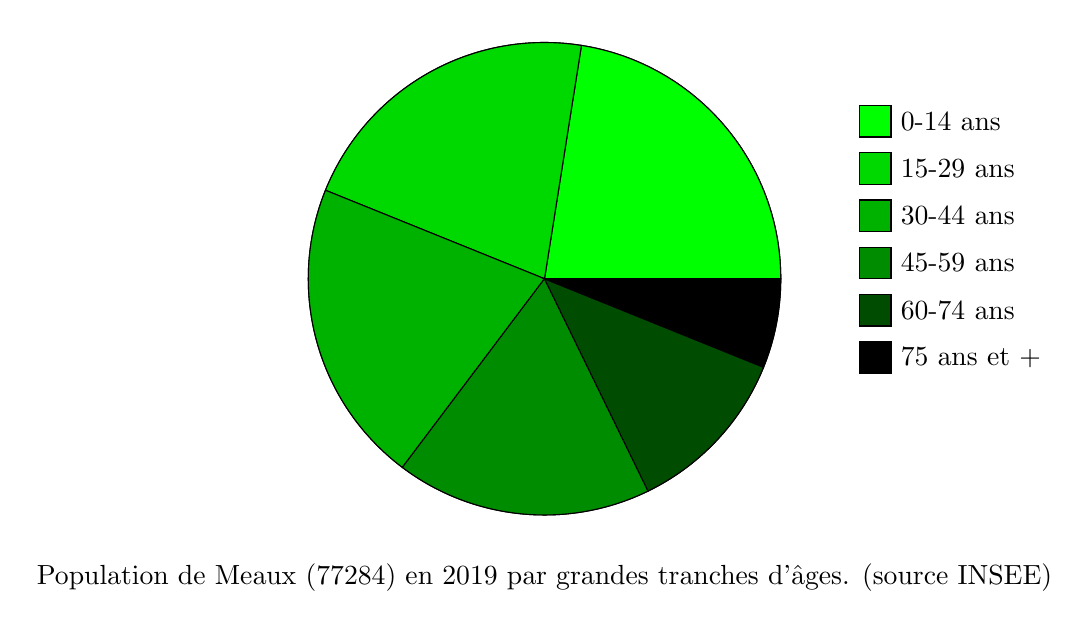
\begin{tikzpicture}
        \draw (0,0) circle (3);
        \draw[fill=green] (0,0) -- (3,0) arc(0:81:3) -- cycle;
        \draw[fill=green!85!black] (0,0) -- ({3*cos(81)},{3*sin(81)}) arc(81:158:3) -- cycle;
        \draw[fill=green!70!black] (0,0) -- ({3*cos(158)},{3*sin(158)}) arc(158:233:3) -- cycle;
        \draw[fill=green!55!black] (0,0) -- ({3*cos(233)},{3*sin(233)}) arc(233:296:3) -- cycle;
        \draw[fill=green!30!black] (0,0) -- ({3*cos(296)},{3*sin(296)}) arc(296:338:3) -- cycle;
        \draw[fill=green!00!black] (0,0) -- ({3*cos(338)},{3*sin(338)}) arc(338:360:3) -- cycle;
        \draw[fill=green] (4,1.8) rectangle ++(0.4,0.4) ++(0,-0.2) node[anchor=west]{0-14 ans};
        \draw[fill=green!85!black] (4,1.2) rectangle ++(0.4,0.4) ++(0,-0.2) node[anchor=west]{15-29 ans};
        \draw[fill=green!70!black] (4,0.6) rectangle ++(0.4,0.4) ++(0,-0.2) node[anchor=west]{30-44 ans};
        \draw[fill=green!55!black] (4,0) rectangle ++(0.4,0.4) ++(0,-0.2) node[anchor=west]{45-59 ans};
        \draw[fill=green!30!black] (4,-0.6) rectangle ++(0.4,0.4) ++(0,-0.2) node[anchor=west]{60-74 ans};
        \draw[fill=green!00!black] (4,-1.2) rectangle ++(0.4,0.4) ++(0,-0.2) node[anchor=west]{75 ans et +};
        \node at (0,-3.8) {Population de Meaux (77284) en 2019 par grandes tranches d'âges. (source INSEE)};
    \end{tikzpicture}
\end{center}    
}

\souspartie{Histogramme}

\definition{Pour représenter des classes de données, on utilise un histogramme où les rectangles sont d'aires proportionnelles aux effectifs des classes.}
\remarque{La hauteur des rectangles est proportionnelle aux effectifs lorsque les classes ont la même étendue.}

\exemple{ (en reprenant les valeurs précédentes)
\begin{center}\color{noir}
    \begin{tikzpicture}
        \draw[-Latex] (0,0) -- (8,0);
        \foreach \x in {0, 15, ..., 75} {
            \draw ({\x/10},-0.1) -- ({\x/10},0.1);
            \node[below] at ({\x/10},-0.1) {\x};
            \draw[-Latex] (0,0) -- (0,5);
        };
        \foreach \x/\d in {0/12585, 1.5/11830, 3/11536, 4.5/9798, 6/6536} {
            \draw[black,fill=gray!50!white] (\x,0) rectangle ({\x+1.5},{\d/3000});
        };
        \foreach \y in {3000, 6000, 9000, 12000} {
            \draw (-0.1,{\y/3000}) -- (0.1,{\y/3000});
            \node[left,anchor=east] at (-0.1,{\y/3000}) {\y};
        }
        \node[anchor=west] at (8,0) {âge};
        \node[anchor=east] at (0,4.5) {effectifs};
    \end{tikzpicture}
\end{center}
}

\partie{Fréquences}

\definition{La fréquence d'une valeur (ou d'une classe de valeurs) dans une série est son effectif divisé par l'effectif total.}

\exemple$
        \item $\dfrac{14}{25} \times 100 = \qty{56}{\%}$
    \end{itemize}
}


\clearpage
\EXERCICES


\end{document}